\chapter{Árvores de sufixos} \label{chap:suffixtree}

\section{Introdução}

\subsection{Suffix tries}

Tries são estruturas poderosas, mas guardam informação apenas sobre os prefixos das strings da coleção de strings que representam. Dada uma string~$P$, se inserirmos todos os sufixos de~$P$ em uma trie, cada caminho nessa trie representará um \emph{prefixo de um sufixo} de~$P$, ou seja, uma substring de~$P$. Se~$T$ é uma trie com todos os sufixos de~$P$, dizemos que~$T$ é a \emph{suffix trie} de~$P$.

Dessa forma, se queremos saber se uma dada string~$S$ ocorre em~$P$, basta checar se é possível percorrer o caminho~$S[1], \tdots, S[|S|]$ na suffix trie de~$P$. Note que isso leva tempo~$\Oh(|S|)$, independente do tamanho de~$P$.

\subsection{Tries comprimidas}

%%%%%% TODO: Escrever melhor ", de um mesmo nó" -> "segue as propriedades", ou algo assim
\begin{definition}
Uma trie comprimida é uma arborescência na qual cada aresta tem um rótulo, que é uma sequência de caracteres, de um mesmo nó não saem duas arestas cujo rótulo começa com o mesmo caractere, e todo nó interno tem grau de saída pelo menos~2.
\end{definition}

Uma trie comprimida é uma generalização de tries em que as arestas podem ser rotuladas por strings em vez de só por caracteres. Para construir uma trie comprimida a partir de uma trie, ``excluímos'' os vértices internos com grau de saída 1, pois podemos juntar o rótulo da aresta que sai deste com o rótulo da aresta que entra nele.
A Figura~\ref{fig:triecomp} mostra como ficaria a trie comprimida da Figura~\ref{fig:triesimple}.

\begin{figure}
\centering
\begin{tikzpicture}[sibling distance=25pt]
\Tree [.{}
[.ma [.mata ] [.ta ] ]
[.o [.ito ] [.mar ] ]
]
\end{tikzpicture}
\caption{Exemplo de trie comprimida.}
\label{fig:triecomp}
\end{figure}

Note que a trie comprimida~$T'$ de~$T$ tem o mesmo número de folhas que~$T$. Seja~$m$ esse número. Como todo vértice interno de~$T'$ tem pelo menos dois filhos, o número de vértices de~$T'$ é no máximo~$2m$. % provar isso será?

\subsection{Suffix tries comprimidas}

Uma suffix trie comprimida de~$P$ é chamada de \emph{árvore de sufixos} de~$P$. Note que, para tries comprimidas, apesar do número de vértices ser não mais que o dobro do número de strings na trie (pois cada string gera no máximo uma folha), o tamanho total das strings nas arestas ainda é proporcional ao tamanho total das strings na trie.

Porém, se temos uma árvore de sufixos de~$P$, e uma aresta tem rótulo~$P[i\tdots j]$, então podemos guardar apenas os índices~$i$ e~$j$ nessa aresta e, assim, como o número de arestas é~$\Oh(|P|)$, temos que a árvore de sufixos de~$P$ pode ser armazenada em espaço~$\Oh(|P|.|\E|)$, usando uma versão adaptada da representação discutida na Seção~\ref{sec:trieimpl}.

Queremos que cada sufixo de~$P$ esteja associado a uma folha dessa árvore, assim não teremos que marcar nós como em tries normais (haveria dificuldade já que nem todo nó da trie está representado nessa árvore). Um sufixo não tem uma folha associada quando é prefixo de outro sufixo. Uma forma simples de forçar isso é criar a árvore de sufixos da string~$P$\$, onde \$ é um caractere que não ocorre na string~$P$. Dessa forma nenhum sufixo é prefixo de outro sufixo e cada sufixo tem uma folha associada.

A Figura~\ref{fig:suftreesimple} mostra a árvore de sufixos da string \texttt{abracadabra}. Note que as arestas estão indicadas como se guardassem uma substring inteira, mas na prática vão guardar apenas dois índices. O rótulo da aresta~$uv$ é mostrado no vértice~$v$.

\begin{figure}[h]
\centering
\begin{tikzpicture}[sibling distance=-1pt]
\Tree [.{}
[.a
    [.bra
        [.cadabra\$ ]
        [.\$ ]
    ]
    [.cadabra\$ ]
    [.dabra\$ ]
    [.\$ ]
]
[.bra
    [.cadabra\$ ]
    [.\$ ]
]
[.cadabra\$ ]
[.dabra\$ ]
[.ra
    [.cadabra\$ ]
    [.\$ ]
]
[.\$ ]
]
\end{tikzpicture}
\caption{Árvore de sufixos para \texttt{abracadabra}.}
\label{fig:suftreesimple}
\end{figure}

\section{Representação}
\label{sec:sufftreerepr}

Para construir a suffix trie de~$P$, basta adicionar cada um dos sufixos de~$P$\$ em uma trie. Mas se queremos criar diretamente a árvore de sufixos de~$P$, existem dificuldades adicionais. É mais complicado navegar na árvore pois em certo ponto podemos estar ``no meio'' de uma aresta, e às vezes pode ser necessário ``quebrar'' uma aresta, para adicionar um vértice no meio desta.

Ao projetar algoritmos para tries, usávamos que~$u(c)$ era o filho de~$u$ por uma aresta rotulada pelo caractere~$c$, ou~\keyword{null} se tal filho não existisse. Para tries comprimidas, usamos que~$u.f[c]$ é o filho de~$u$ por uma aresta cujo rótulo tem \emph{primeiro} caractere~$c$, ou~\keyword{null} se tal filho não existir. Além disso, é necessário guardar mais informação sobre as arestas, e para a aresta~$uv$ guardamos essa informação no vértice~$v$, ou seja, em cada nó guardamos os dados sobre a aresta incidente neste.

Seja~$e = uv$ a aresta que chega em~$v$. Guardamos em~$v.p$ o identificador de~$u$. Os campos~$v.l$ e~$v.r$ guardam os índices que determinam o rótulo~$P[l\tdots r]$ da aresta~$e$. Baseados nesses valores, escrevemos~${v.s[i] = P[v.l + i - 1]}$ para acessar o~$i$-ésimo caractere do rótulo de~$e$, e~${\len{v} = v.r - v.l + 1}$ para o tamanho do rótulo de~$e$, para deixar o código mais limpo. Usamos~${\textbf{new } \node(l, r, p)}$ para representar a criação de uma aresta que sai de~$p$ e tem rótulo~$P[l\tdots r]$, se ligando a um novo vértice. Como convenção a raiz é inicializada com~$\textbf{new } \node(1, 0, \textbf{ null})$, ou seja, sua ``aresta'' está rotulada pela string vazia.

Seja~$T$ uma trie, e~$T_c$ a trie comprimida associada. Para navegar em~$T$, é suficiente guardar uma variável~$u$ que representa o nó atual que o algoritmo está analisando. Em~$T_c$ usaremos duas variáveis,~$\cn$ e~$\cd$, onde~$\cn$ é um vértice em~$T_c$, e~$\cd$ um inteiro que determina quantos caracteres do rótulo da aresta de~$\cn.p$ para~$\cn$ já percorremos. O par~$(\cn, \cd)$ determina unicamente um vértice em~$T$. Note que se~$\cd = \len{\cn}$ então estamos exatamente no vértice~$\cn$, e não no meio de uma aresta.
 
\section{Construção em tempo quadrático}
O algoritmo no Código~\ref{lst:sufftreequad} mostra como construir a árvore de sufixos de~$P$ em tempo~$\Oh(|P|^2)$, usando memória~$\Oh(|P|.|\E|)$. Apresentamos esse código aqui pois pode ser útil para strings pequenas, já que é mais fácil de entender e implementar que o código que vamos apresentar na Seção~\ref{sec:sufftreelin}, que consome tempo linear. Ele também deixa claro como utilizamos a forma de representação discutida na Seção~\ref{sec:sufftreerepr}. 

A função~\func{BuildSuffixTreeQuad}{P} constrói a árvore de sufixos da string~$P$, adicionando cada sufixo de~$P$ em uma trie comprimida. A árvore de sufixos inicialmente consiste só da raiz~$r$, inicializada como discutido acima. 

% fazer retornar a raiz
\begin{algorithm}
\caption{Árvore de sufixos em tempo quadrático}
\label{lst:sufftreequad}
\begin{algorithmic}[1]
\Function {BuildSuffixTreeQuad}{$P$}
    \State $P \pluseq \text{`\$'}$
    \For {$i = 1 \To |P|$}
        \State $\cn = r$
        \State $\cd = 0$
        \For {$j = i \To |P|$}
            \If {$\cd = \len{\cn} \And \cn.f[P[j]] = \Null$} \Comment{Não é necessário quebrar a aresta}
                \State $\cn.f[P[j]] = \New \node(j, |P|, \cn)$
                \State \Break
            \EndIf
            \If {$\cd < \len{\cn} \And \cn.s[\cd + 1] \neq P[j]$} \Comment{Quebrando a aresta}
                \State $\mmid = \New \node(\cn.l, \cn.l + \cd - 1, \cn.p)$
                \State $\cn.p.f[\mmid.s[1]] = \mmid$ 
                \State $\mmid.f[\cn.s[\cd + 1]] = \cn$
                \State $\cn.p = \mmid$
                \State $\cn.l \pluseq \cd$
                \State $\mmid.f[P[j]] = \New \node(j, |P|, \mmid)$
                \State \Break
            \EndIf
            \If {$\cd = \len{\cn}$} \Comment{Percorrendo 1 caractere}
                \State $\cn = \cn.f[P[j]]$
                \State $\cd = 0$
            \EndIf
            \State $\cd \pluseq 1$
        \EndFor
    \EndFor
\EndFunction
\end{algorithmic}
\end{algorithm}

\pagebreak
\begin{invar}
No início da iteração~$j$ do \keyword{for} da linha 6, o par~$(\cn, \cd)$ indica o nó (na trie não comprimida) que tem como string associada~$P[i\tdots j-1]$.
\end{invar}

\begin{proof}
Quando~$j = i$, o invariante vale pois a raiz é associada à string vazia e o par~$(\cn, \cd)$ é iniciado corretamente nas linhas 4-5.

Suponha que o invariante vale no início da iteração~$j$. Os \keyword{if}s das linhas 7 e~10 verificam se não existe caminho a partir do nó atual com caractere~$P[j]$, e se algum deles executar, o \keyword{for} é terminado.

Se os \keyword{if}s não executarem, então se~$\cd < \len{\cn}$ sabemos que o~$(\cd+1)$-ésimo caractere na aresta incidente em~$\cn$ é~$P[j]$, e assim podemos incrementar~$\cd$ em~$1$ para representar o vértice associado a~$P[i\tdots j]$. Se~$\cd = \len{\cn}$ sabemos que existe aresta com primeiro caractere~$P[j]$ saindo de~$\cn$, assim as linhas 19-20 fazem~$\cn$ apontar para o vértice no final dessa aresta, e~$\cd$ é inicializado com~$0$ e depois incrementado para~$1$, assim representando a string~$P[i\tdots j]$.

Assim os novos valores de~$(\cn, \cd)$ indicam o nó associado a~$P[i\tdots j]$, e o invariante vale na próxima iteração.
\end{proof}

Pelo invariante, temos que o \keyword{for} nas linhas 6-21 percorre o maior prefixo de~$P[i\tdots |P|]$ que já está na árvore de sufixos. Se este terminar normalmente, então o sufixo~$P[i\tdots |P|]$ já está na árvore de sufixos, senão os casos são tratados pelos \keyword{if}s das linhas 7 e~10 da seguinte forma:

\begin{figure}
\centering
\tikzstyle{circlee} = [circle, minimum size=1cm, text centered, draw=black]
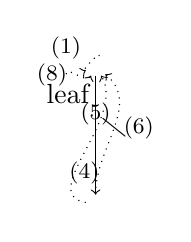
\begin{tikzpicture}[sibling distance=50pt, level distance=40pt,every tree node/.style=circlee,
edge from parent path={(\tikzparentnode) -- (\tikzchildnode)}]
\Tree [.\node(root){};
\edge[->] node[midway, right]{\footnotesize (2)}; [.\node(mid){$\mmid$}; \edge[->] node[midway,right,xshift=-2pt]{\footnotesize (7)}; [.\node(leaf)[xshift=-10pt, yshift=-10pt]{leaf}; ] ]
\edge[->] node[midway, left,yshift=5pt]{\footnotesize (3)} node[pos=0.5,sloped]{/}; [.\node[yshift=-50pt](cn){$\cn$}; ]
]


\draw[->] (mid) -- (cn) node[midway, above]{\footnotesize (5)};
\draw[dotted,->] (cn) to[out=170,in=-60] node[midway, below]{\footnotesize (4)} (mid);

\draw[dotted,->] (leaf) to[out=95,in=-115] node[midway, left]{\footnotesize (8)} (mid);

\draw[dotted,->] (mid) to[out=70,in=205] node[midway, left,yshift=5pt]{\footnotesize (1)} (root);

\draw[dotted,->] (cn) to[out=90, in=-40] node[midway, right]{\footnotesize (6)} node[pos=0.5,sloped]{/} (root);
\end{tikzpicture}
\caption{Inserção de~$\mmid$.} \label{fig:midinsert}
\end{figure}

\begin{description}
    \item[Linha 7.] Se~$\cd = \len{\cn}$ e nenhuma aresta sai de~$\cn$ com primeiro caractere~$P[j]$ então não existe caminho, e nesse caso basta criar uma nova folha apontada por~$\cn$ associada ao sufixo~$P[j\tdots |P|]$.
    
    \item[Linha 10.] Se~$\cd < \len{\cn}$ e o próximo caractere da aresta incidente em~$\cn$ é diferente de~$P[j]$ então não existe caminho, e nesse caso é necessário quebrar esta aresta em duas neste ponto, sendo uma para os primeiros~$\cd$ caracteres e outra para o restante. A partir do novo vértice, cria-se uma aresta associada ao sufixo~$P[j\tdots |P|]$. Essa quebra de aresta é a parte mais complicada do algoritmo, e será explicada usando a Figura~\ref{fig:midinsert}. Os links guardados na lista de adjacência (variável~$f$) de cada vértice são representadas com arestas cheias, e os links de pai guardadas na variável~$p$ são representadas por arestas pontilhadas.
    
    Inicialmente apenas os links~(3) e~(6) existem. A linha 11 cria o vértice~$\mmid$ e o link (1). A linha 12 apaga o link~(3) e cria o link (2), pois apesar de criarmos~$\mmid$ como filho de~$\cn.p$, na lista de adjacência desse vértice não é atualizada pela função~$\textbf{new } \node$. As linhas~13 e~14 fazem~$\cn$ ser filho de~$\mmid$, criando o link~(5), apagando o link~(6) e criando o link (4). A linha~15 apenas atualiza o rótulo da aresta que chega em~$\cn$, removendo os~$\cd$ primeiros caracteres, e finalmente a linha~16 cria a nova folha e assim os links (7) e (8).
\end{description}

%%%%%%%%%%%%%%%%%%%%%%%%%%%%%%%%%%%%%%%%%
%%%%%% CONSTRUCAO BANANA %%%%%%%%%%%%%%%%
%%%%%%%%%%%%%%%%%%%%%%%%%%%%%%%%%%%%%%%%%
\begin{figure}

\subfloat[\texttt{banana\$}] {
\begin{minipage}{0.5\textwidth}
\centering
\begin{tikzpicture}
\Tree [.{}
[.banana\$ ]
]
\end{tikzpicture}
\end{minipage}}
\hfill
\subfloat[\texttt{anana\$}]{
\begin{minipage}{0.5\textwidth}
\centering
\begin{tikzpicture}
\Tree [.{}
[.anana\$ ]
[.banana\$ ]
]
\end{tikzpicture}
\end{minipage}}
\hfill
\subfloat[\texttt{nana\$}]{
\begin{minipage}{0.5\textwidth}
\centering
\begin{tikzpicture}
\Tree [.{}
[.anana\$ ]
[.banana\$ ]
[.nana\$ ]
]
\end{tikzpicture}
\end{minipage}}
\hfill
\subfloat[\texttt{ana\$}]{
\begin{minipage}{0.5\textwidth}
\centering
\begin{tikzpicture}
\Tree [.{}
[.ana [.na\$ ] [.\$ ] ]
[.banana\$ ]
[.nana\$ ]
]
\end{tikzpicture}
\end{minipage}}
\hfill
\subfloat[\texttt{na\$}]{
\begin{minipage}{0.5\textwidth}
\centering
\begin{tikzpicture}
\Tree [.{}
[.ana [.na\$ ] [.\$ ] ]
[.banana\$ ]
[.na [.na\$ ] [.\$ ] ]
]
\end{tikzpicture}
\end{minipage}}
\hfill
\subfloat[\texttt{a\$}]{
\begin{minipage}{0.5\textwidth}
\centering
\begin{tikzpicture}
\Tree [.{}
[.a [.na [.na\$ ] [.\$ ] ] [.\$ ] ]
[.banana\$ ]
[.na [.na\$ ] [.\$ ] ]
]
\end{tikzpicture}
\end{minipage}}
\hfill
\subfloat[\texttt{\$}]{
\begin{minipage}{\textwidth}
\centering
\begin{tikzpicture}
\Tree [.{}
[.a [.na [.na\$ ] [.\$ ] ] [.\$ ] ]
[.banana\$ ]
[.na [.na\$ ] [.\$ ] ]
[.\$ ]
]
\end{tikzpicture}
\end{minipage}}


\caption{Construção da árvore de sufixos de \texttt{banana} em tempo quadrático.}
\label{fig:bananaquad}
\end{figure}
%%%%%%%%%%%%%%%%%%%%%%%%%%%%%%%%%%%%%%%%%
%%%%%% FIM CONSTRUCAO BANANA %%%%%%%%%%%%
%%%%%%%%%%%%%%%%%%%%%%%%%%%%%%%%%%%%%%%%%

Logo, o sufixo~$P[i\tdots |P|]$ é adicionado corretamente à árvore de sufixos. Como todos os sufixos são adicionados pelo \keyword{for} da linha 3, então a função \mbox{\func{BuildSuffixTreeQuad}{P}} funciona corretamente. Note que como adicionamos um caractere \$ ao final de~$P$, nenhum sufixo é prefixo de outro sufixo, logo uma destas condições sempre acontece ao adicionar cada sufixo. A Figura~\ref{fig:bananaquad} mostra a construção de uma árvore de sufixos para \texttt{banana} usando o algoritmo apresentado nessa seção, adicionando sufixo por sufixo.

\section{Uso}


O Código~\ref{lst:sufftreequad} também mostra como percorrer a árvore de sufixos, e com isto já é possível determinar se~$S$ ocorre em~$P$ em tempo~$\Oh(|S|)$. Basta verificar se é possível seguir o caminho~$S[1], \ldots, S[|S|]$ na árvore de sufixos de~$P$. Se em cada vértice da árvore de sufixos guardarmos o número de folhas que estão em sua subárvore (pode ser facilmente feito com uma busca em profundidade (DFS) em tempo~$\Oh(|P|.|\E|)$), também teremos o número de ocorrências de~$S$ em~$P$, pois cada folha alcançável indica uma ocorrência no começo do sufixo associado a esta folha. Aqui, estamos usando o fato de nossa árvore ter uma folha para cada sufixo de~$P$. Note que se o final de~$S$ está no meio de uma aresta, o número de folhas atingíveis é o mesmo que se seguirmos essa aresta até o final.

É possível ainda descobrir quais são essas ocorrências em tempo proporcional ao número destas, apenas percorrendo (com uma DFS, por exemplo) a subárvore do vértice que representa~$S$, pois o número de nós nesta subárvore é proporcional ao número de folhas. Observe que devemos percorrê-la como uma árvore normal, ignorando que as arestas podem ter um rótulo extenso, assim cada aresta é percorrida em tempo~$\Oh(1)$ e o tempo de visitar as folhas fica proporcional ao número destas.

Note que se tivermos uma árvore de sufixos de~$P$, conseguimos realizar o mesmo que com o algoritmo de Aho-Corasick, pois para um conjunto~$\cS = \{S_1, \ldots, S_k\}$ de strings, podemos descobrir as ocorrências de cada string de~$\cS$ em tempo~$\Oh(\sum\limits_{i=1}^k{|S_i|} + x)$, onde~$x$ é o número dessas ocorrências, usando o algoritmo descrito acima para cada uma das strings. Na próxima seção apresentaremos a criação de uma árvore de sufixos em tempo linear, e assim será possível atingir o mesmo tempo que Aho-Corasick, sem precisar ter acesso às strings de~$\cS$ de antemão. O código, contudo, é mais complicado que o do Aho-Corasick.







\section{Construção em tempo linear}
\label{sec:sufftreelin}

O primeiro algoritmo para criação de árvores de sufixos em tempo linear foi proposto por Weiner~\cite{weiner}, mas o algoritmo que apresentaremos será o algoritmo de Ukkonen~\cite{ukkonen}, por ser mais simples.


A ideia deste algoritmo é adicionar um prefixo de~$P$ por vez, segundo a ordem~$P[1\tdots 1], P[1\tdots 2], \ldots, P[1\tdots |P|]$. Dessa forma temos um algoritmo \emph{online}, ou seja, não é necessário ter a string~$P$ inteira inicialmente. Ela pode ser dada caractere por caractere.

Vamos definir~$T_j$ como a árvore de sufixos para~$P[1\tdots j]$.
Na~$j$-ésima iteração, temos~$T_{j-1}$ e queremos, a partir desta, construir~$T_j$. Para isso adicionamos os sufixos~$P[1\tdots j], P[2\tdots j], \ldots, P[j\tdots j]$, nesta ordem. Para~$1 \leq i \leq j$, ao adicionarmos~$P[i\tdots j]$, dizemos que estamos realizando a~$i$-ésima extensão na~$j$-ésima iteração. Note que, pela descrição, esse algoritmo leva tempo~$\Oh(n^3)$, potencialmente pior que o algoritmo simples descrito na seção anterior. Mas com algumas otimizações é possível diminuir seu tempo para~$\Oh(n)$.

\begin{definition}
Dizemos que uma string~$S$ \textbf{está} na árvore de sufixos~$T$ se existe um caminho a partir da raiz de~$T$ no qual a string associada é~$S$.
\end{definition}

\begin{lemma}
\label{lem:caso1}
Se alguma string~$S$ está na árvore de sufixos~$T$, então todos os sufixos de~$S$ também estão.
\end{lemma}

\begin{proof}
Como~$T$ é uma árvore de sufixos de alguma string~$P$, a string~$S$ é uma substring de~$P$ (pois todo caminho a partir da raiz de~$T$ representa uma substring de~$P$). Mas todo sufixo de~$S$ também é uma substring de~$P$, e assim está representado em~$T$.
\end{proof}

\begin{lemma}
\label{lem:caso4}
Para~$1 \leq i \leq j$, se o nó associado a~$P[i\tdots j]$ é uma folha em~$T_j$, então~$P[i\tdots j+1]$ \emph{não} está representado em~$T_j$. Ao adicionar~$P[i\tdots j+1]$, esse também será associado a uma folha no final da~$(j+1)$-ésima iteração.
\end{lemma}

\begin{proof}
Como~$P[i\tdots j] \prefp P[i\tdots j+1]$, o caminho para~$P[i\tdots j+1]$ passa pelo nó associado a~$P[i\tdots j]$. Mas este é uma folha, logo~$P[i\tdots j + 1]$ não está em~$T_j$.

Ao ser adicionado,~$P[i\tdots j+1]$ é uma folha, pois basta adicionar o caractere~$P[j+1]$ na aresta que chega na folha de~$P[i\tdots j]$. Para mostrar que este vértice continua uma folha ao final da~$(j+1)$-ésima iteração, basta mostrar que nenhuma outra string adicionada nessa iteração tem~$P[i\tdots j+1]$ como prefixo. Suponha que~$P[i\tdots j+1] \prefp P[k\tdots j+1]$, para algum~$k$. Então~$P[i\tdots j] \prefp P[k\tdots j]$. Mas~$P[i\tdots j]$ é uma folha, e~$P[k\tdots j]$ é uma string maior que~$P[i\tdots j]$ que tem esta como prefixo, o que leva a uma contradição pois~$P[k\tdots j]$ já estava em~$T_j$.
\end{proof}

Ao executar a~$i$-ésima extensão na~$j$-ésima iteração, estamos adicionando a substring~$P[i\tdots j]$ a~$T_{j-1}$. Então claramente já existe caminho associado a~$P[i\tdots j-1]$. Logo resta apenas adicionar o caractere~$P[j]$ a esse caminho. Existem quatro casos possíveis:

\begin{description}
    \item [Caso 1.] O caminho~$P[i\tdots j]$ já existe em~$T_{j-1}$. Nesse caso nada precisa ser feito.
    \item [Caso 2.] O caminho~$P[i\tdots j-1]$ termina em um vértice não-folha. Nesse caso basta criar uma folha conectada a esse vértice por uma aresta associada a~$P[j]$.
    \item [Caso 3.] O caminho~$P[i\tdots j-1]$ termina em uma aresta (pois as arestas de uma árvore de sufixos podem ser associadas a rótulos com mais de um caractere). Nesse caso, é necessário ``quebrar'' a aresta, ou seja, criar um vértice interno no meio dessa aresta e, a partir deste ponto, é como no caso anterior.
    \item [Caso 4.] O caminho~$P[i\tdots j-1]$ termina em uma folha. Nesse caso basta apenas ``estender'' essa folha, ou seja, aumentar em um o tamanho da aresta que chega nessa folha.
\end{description}

\begin{theorem}
\label{thm:estcasos}
Para~$1 \leq i \leq j$, seja~$C(i, j)$ o caso que ocorreu na~$i$-ésima extensão da~$j$-ésima iteração. Para todo~$1 \leq j \leq |P|$, a sequência~$C(1, j), C(2, j), \ldots, C(j, j)$ se comporta da seguinte maneira:
\begin{itemize}
    \item Há um prefixo de~$4$'s.
    \item Após esse prefixo, há uma sequência de~$3$'s ou~$2$'s.
    \item Após essa sequência, há um sufixo de~$1$'s.
\end{itemize}
Além disso, para~$j > 1$,~$C(i, j) = 4$ se e somente se~$C(i, j - 1) \neq 1$.
\end{theorem}

\begin{proof}
Vamos provar o teorema por indução em~$j$, ou seja, vamos provar por indução em~$j$ que a sequência~$C(1, j), \ldots, C(j, j)$ satisfaz os três itens do teorema e a observação que segue. A base,~$j = 1$, é fácil: a árvore~$T_0$ só tem a raiz então~$C(1, 1) = 2$, pois considera-se que a raiz não é uma folha, mesmo quando sozinha.

Para~$j > 1$, suponha por indução que~$C(1, j-1), \ldots, C(j-1, j-1)$ satisfaz as condições do teorema. Vamos mostrar que as condições valem para~$j$.
Para~${1 \leq i < j}$, se~$C(i, j - 1) = 4$, pelo Lema~\ref{lem:caso4} temos que~$C(i, j) = 4$ também. O mesmo vale se~${C(i, j - 1) \in \{2, 3\}}$, pois esses casos levam à criação de folhas. Então o prefixo de~$4$'s,~$3$'s e~$2$'s de~$C(1, j-1), \ldots, C(j - 1, j - 1)$ correspondem a um prefixo de~$4$'s de~$C(1, j), \ldots, C(j - 1, j)$.

Para~$1 \leq i \leq j$, o Lema~\ref{lem:caso1} nos diz que se~$P[i\tdots j]$ está na árvore de sufixos, então~${P[i+1\tdots j], \ldots, P[j\tdots j]}$ também estão. Isso é equivalente a dizer que se~$C(i, j) = 1$, então~$C(i + 1, j) = \cdots = C(j, j) = 1$, logo, a sequência de~$1$'s forma um sufixo.

Note que resta apenas mostrar que~$C(i, j) \neq 4$ se~$C(i, j - 1) = 1$ ou se~$i = j$. Se~$i = j$, isso vale pois~$P[i\tdots i-1]$ termina na raiz, que não é uma folha. Se~$i < j$ então, se~$C(i, j - 1) = 1$, temos que a string~$P[i\tdots j-1]$ já estava na árvore~$T_{j-2}$ quando foi inserida na~$i$-ésima extensão da~${(j-1)\text{-ésima}}$ iteração. Assim~${P[i\tdots j-1] = P[i-k\tdots j-1-k]}$, para algum~$k > 0$, e nesse caso~$P[i-k\tdots j-1-k] \prefp P[i-k\tdots j-1]$. Logo~$P[i\tdots j-1]$ não é uma folha e~$C(i, j) \neq 4$.
\end{proof}

Com esse teorema, é possível realizar apenas~$\Oh(|P|)$ extensões para criar~$T_{|P|}$. As operações feitas no caso~$4$ podem ser feitas automaticamente. Basta, nas folhas, em vez de guardar~$l$ e~$r$ normalmente para indicar a string~$P[l\tdots r]$, no valor de~$r$ guardarmos um valor especial (como~$-1$ ou algum valor maior que~$|P|$) indicando que o valor real de~$r$ é o número da iteração atual. Porém, só é necessário que o comprimento do rótulo sempre seja maior ou igual ao valor que teria se~$r$ fosse igual ao número da iteração atual. Logo, podemos guardar~$|P|$ nos valores de~$r$ da folha. O algoritmo funcionará e esses campos estarão corretos quando o algoritmo acabar.

Dessa forma, não é necessário fazer nada no caso 4. Precisamos apenas começar da primeira ocorrência do caso 1 da iteração~$j-1$, ou de~$j$ se o caso 1 não tiver ocorrido na iteração~$j-1$. Quando ocorre um caso~1 na iteração~$j$, sabemos que todas as próximas extensões nessa iteração serão do caso~1. Portanto não é necessário executar o resto da iteração e podemos ir para a iteração~$j + 1$. Assim, no máximo um índice de extensão é analisado em duas iterações consecutivas (se ocorreu caso~1 na primeira destas iterações), e executamos no máximo~$2|P|$ extensões entre todas as iterações.

\begin{algorithm}
\caption{Árvore de sufixos em tempo linear}
\label{lst:sufftreelin}
\begin{algorithmic}[1]
\Function{BuildSuffixTree}{$P$}
    \State $P \pluseq \text{`\$'}$
    \State $r = \New \node(1, 0, \Null)$ \Comment{raiz inicializada com rótulo vazio}
    \State $(i, \cn, \cd, \ns) = (1, r, 0, \Null)$
    \For{$j = 1 \To |P|$} \label{lst:stl:mainfor} \Comment{$j$-ésima iteração}
        \While{$i \leq j$} \label{lst:stl:mainwhile} \Comment{$i$-ésima extensão}
            \If{$\cd = \len{\cn} \And \cn.f[P[j]] \neq \Null$} \label{lst:stl:caso1s} \Comment{caso 1}
                \State $\cn = \cn.f[P[j]]$ \label{lst:stl:cn1}
                \State $\cd = 0$ \label{lst:stl:caso1.2}
            \EndIf
            \If{$\cd < \len{\cn} \And \cn.s[\cd + 1] = P[j]$} \label{lst:stl:caso1.1}
                \State $\cd \pluseq 1$ \label{lst:stl:incrcd}
                \State \Break \label{lst:stl:caso1e}
            \EndIf
            \If{$\cd = \len{\cn}$} \label{lst:stl:caso2s} \Comment{caso 2}
                \State $\cn.f[P[j]] = \New \node(j, |P|, \cn)$
                \If{$\cn \neq r$}
                    \State $\cn = \cn.\suf$ \label{lst:stl:cn2}
                    \State $\cd = \len{\cn}$ \label{lst:stl:caso2e}
                \EndIf
            \Else \label{lst:stl:caso3s} \Comment{caso 3}
                \State $\mmid = \New \node(\cn.l, \cn.l + \cd - 1, \cn.p)$ \label{lst:stl:mids}
                \State $\cn.p.f[\mmid.s[1]] = \mmid$ 
                \State $\mmid.f[\cn.s[\cd + 1]] = \cn$ \label{lst:stl:midcns}
                \State $\cn.p = \mmid$
                \State $\cn.l \pluseq \cd$  \label{lst:stl:midcne}
                \State $\mmid.f[P[j]] = \New \node(j, |P|, \mmid)$ \label{lst:stl:leaf} \label{lst:stl:mide}
                \If{$\ns \neq \Null$} \label{lst:stl:sufs}
                    \State $\ns.\suf = \mmid$ \label{lst:stl:sufe}
                \EndIf
%                \algstore{sufflin}
%\end{algorithmic}
%\end{algorithm}
%
%\begin{algorithm}
%\begin{algorithmic}[1]
%                \algrestore{sufflin}
                \State $\cn = \mmid.p$ \label{lst:stl:buscas} \label{lst:stl:cn3}
                \If{$\cn \neq r$}
                    \State $\cn = \cn.\suf$ \label{lst:stl:cn4}
                    \State $g = j - \cd$ \label{lst:stl:g1}
                \Else \Comment{No início do laço,~$\cn$ está associado a~$P[i+1\tdots g-1]$}
                    \State $g = i + 1$ \label{lst:stl:cninite} \label{lst:stl:g2}
                \EndIf 
                \While{$g < j \And g + \len{\cn.f[P[g]]} \leq j$} \label{lst:stl:whileauxs}
                    \State $\cn = \cn.f[P[g]]$ \label{lst:stl:edge} \label{lst:stl:cn5}
                    \State $g \pluseq \len{\cn}$ \label{lst:stl:whileauxe} \label{lst:stl:g3}
                \EndWhile
                \If{$g = j$}
                    \State $\ns = \Null$ \label{lst:stl:midsufs}
                    \State $\mmid.\suf = \cn$ \label{lst:stl:midsufe}
                    \State $\cd = \len{\cn}$
                \Else
                    \State $\ns = \mmid$ \label{lst:stl:midns}
                    \State $\cn = \cn.f[P[g]]$ \label{lst:stl:cncds} \label{lst:stl:cn6}
                    \State $\cd = j - g$  \label{lst:stl:caso3e}
                \EndIf
            \EndIf
            \State $i \pluseq 1$
        \EndWhile
    \EndFor
    \State $\Return$~$r$
\EndFunction
\end{algorithmic}
\end{algorithm}


O Código~\ref{lst:sufftreelin} mostra como criar uma árvore de sufixos para uma string~$P$ em tempo linear. O \keyword{for} na linha~\nref{lst:stl:mainfor} executa cada uma das iterações e o \keyword{while} na linha~\nref{lst:stl:mainwhile} executa cada uma das extensões. A otimização discutida acima está implementada, e assim são feitas apenas~$\Oh(|P|)$ extensões.
As variáveis~$\cn$ e~$\cd$ são usadas como anteriormente para navegar pela árvore. O novo campo~$v.\suf$, chamado de \emph{link de sufixo} de~$v$, representa, para um vértice interno (não-folha e não-raiz)~$v$ associado a~$P[i\tdots j]$, o vértice~$u$ associado a~$P[i+1\tdots j]$, ou seja, à string de~$v$ sem o primeiro caractere.
Esse valor é usado para navegar mais rapidamente pela árvore, como mostraremos adiante. A variável~$\ns$ é uma variável auxiliar na criação dos links de sufixo, e indica o único nó interno que está com o valor de~$\suf$ indefinido, quando há um.

%%%%%%%%%%%%%%%%%%%%%%%%%%%%%%%%%%%%%%%%%
%%%%%% CONSTRUCAO BANANA %%%%%%%%%%%%%%%%
%%%%%%%%%%%%%%%%%%%%%%%%%%%%%%%%%%%%%%%%%
\begin{figure}
\subfloat[(1, 1) Caso 2] {
\begin{minipage}{0.3\textwidth}
\centering
\begin{tikzpicture}
\Tree [.{}
[.b ]
]
\end{tikzpicture}
\end{minipage}
}
\hfill
\subfloat[(2, 2) Caso 2]{
\begin{minipage}{0.3\textwidth}
\centering
\begin{tikzpicture}
\Tree [.{}
[.a ]
[.ba ]
]
\end{tikzpicture}
\end{minipage}
}
\hfill
\subfloat[(3, 3) Caso 2]{
\begin{minipage}{0.3\textwidth}
\centering
\begin{tikzpicture}
\Tree [.{}
[.an ]
[.ban ]
[.n ]
]
\end{tikzpicture}
\end{minipage}
}
\hfill
\subfloat[(4, 4) Caso 1]{
\begin{minipage}{0.3\textwidth}
\centering
\begin{tikzpicture}
\Tree [.{}
[.ana ]
[.bana ]
[.na ]
]
\end{tikzpicture}
\end{minipage}
}
\hfill
\subfloat[(4, 5) Caso 1]{
\begin{minipage}{0.3\textwidth}
\centering
\begin{tikzpicture}
\Tree [.{}
[.anan ]
[.banan ]
[.nan ]
]
\end{tikzpicture}
\end{minipage}}
\hfill
\subfloat[(4, 6) Caso 1]{
\begin{minipage}{0.3\textwidth}
\centering
\begin{tikzpicture}
\Tree [.{}
[.anana ]
[.banana ]
[.nana ]
]
\end{tikzpicture}
\end{minipage}
}
\hfill
\subfloat[(4, 7) Caso 3]{
\begin{minipage}{0.45\textwidth}
\centering
\begin{tikzpicture}
\Tree [.{}
[.ana [.na\$ ] [.\$ ] ]
[.banana\$ ]
[.nana\$ ]
]
\end{tikzpicture}
\end{minipage}
}
\hfill
\subfloat[(5, 7) Caso 3]{
\begin{minipage}{0.45\textwidth}
\centering
\begin{tikzpicture}
\Tree [.{}
[.ana [.na\$ ] [.\$ ] ]
[.banana\$ ]
[.na [.na\$ ] [.\$ ] ]
]
\end{tikzpicture}
\end{minipage}
}
\hfill
\subfloat[(6, 7) Caso 3]{
\begin{minipage}{0.45\textwidth}
\centering
\begin{tikzpicture}
\Tree [.{}
[.a [.na [.na\$ ] [.\$ ] ] [.\$ ] ]
[.banana\$ ]
[.na [.na\$ ] [.\$ ] ]
]
\end{tikzpicture}
\end{minipage}
}
\hfill
\subfloat[(7, 7) Caso 2]{
\begin{minipage}{0.45\textwidth}
\centering
\begin{tikzpicture}
\Tree [.{}
[.a [.na [.na\$ ] [.\$ ] ] [.\$ ] ]
[.banana\$ ]
[.na [.na\$ ] [.\$ ] ]
[.\$ ]
]
\end{tikzpicture}
\end{minipage}
}


\caption{Construção da árvore de sufixos de \texttt{banana} em tempo linear.}
\label{fig:bananalin}
\end{figure}
%%%%%%%%%%%%%%%%%%%%%%%%%%%%%%%%%%%%%%%%%
%%%%%% FIM CONSTRUCAO BANANA %%%%%%%%%%%%
%%%%%%%%%%%%%%%%%%%%%%%%%%%%%%%%%%%%%%%%%


A Figura~\ref{fig:bananalin} mostra a construção da árvore de sufixos de \texttt{banana} com o algoritmo do Código~\ref{lst:sufftreelin}, mostrando o resultado depois de cada extensão realizada. Os números em parênteses mostram respectivamente a extensão e a iteração atual. A árvore é mostrada com as aplicações do caso 4 implícitas, ou seja, apesar de as folhas terem valor de~$r$ como~$|P|$, mostramos como se o valor fosse o da iteração atual.

\pagebreak
\begin{invar}
No começo da~$i$-ésima iteração do \keyword{while} da linha~\nref{lst:stl:mainwhile}, na~$j$-ésima iteração do \keyword{for}, o par~$(\cn, \cd)$ indica o vértice (ou aresta) que representa a substring~${P[i\tdots j-1]}$. Nesse ponto, a árvore de sufixos é~$T_{j-1}$ com as strings~$P[1\tdots j], \ldots, P[i-1\tdots j]$ adicionadas.

Além disso, sempre que um vértice interno for criado (por uma aplicação do caso 3), o seu link de sufixo será definido antes do final da próxima extensão. Enquanto um nó tiver o valor de~$\suf$ indefinido, seu valor será guardado na variável~$\ns$.
\end{invar}

\begin{proof}
Na primeira iteração do \keyword{while} da linha~\nref{lst:stl:mainwhile}, estamos na primeira extensão da primeira iteração, ou seja, queremos adicionar a substring~$P[1\tdots 1]$, e o par~$(\cn, \cd)$ inicialmente indica a raiz, que está associada à string vazia, e o invariante vale.

No começo da iteração, estamos na substring~$P[i\tdots j-1]$ e queremos adicionar o caractere~$P[j]$. Como discutido anteriormente, isso se reduz a quatro casos. As linhas~${\nref{lst:stl:caso1s}\text{-}\nref{lst:stl:caso1e}}$ tratam o caso~1; as linhas~\nref{lst:stl:caso2s}-\nref{lst:stl:caso2e} tratam o caso~2; as linhas~\nref{lst:stl:caso3s}-\nref{lst:stl:caso3e} tratam o caso~3; o caso~4 nunca é tratado explicitamente, pois sempre estamos em uma extensão em que ocorre um dos demais casos.

Se~$\cd < \len{\cn}$, dizemos que a substring representada pelo par~$(\cn, \cd)$ é interna, ou seja, acaba ``no meio'' de uma aresta.

O caso~$1$ ocorre quando a substring~$P[i\tdots j - 1]$ é interna e a aresta à qual pertence continua com o caractere~$P[j]$, tratado nas linhas~\nref{lst:stl:caso1.1}-\nref{lst:stl:caso1e}, ou quando~$P[i\tdots j - 1]$ não é interna e o vértice em que acaba tem uma aresta que começa com~$P[j]$. Nesse caso seguimos ``0'' caracteres na direção dessa aresta (linhas~${\nref{lst:stl:caso1s}\text{-}\nref{lst:stl:caso1.2}}$) e o caso pode ser tratado como se fosse o anterior. Se ocorrer o caso~1, a substring~$P[i\tdots j]$ já existe na árvore, e a iteração~$j$ acaba. A próxima extensão vai ser a~$i$-ésima extensão da~$(j+1)$-ésima iteração (pela otimização discutida anteriormente), ou seja, vamos adicionar a string~$P[i\tdots j+1]$. Para manter o invariante, é necessário avançar para a string~$P[i\tdots j]$, ou seja, basta seguir o caminho que sabemos que existe, ou continuando na aresta se~$P[i\tdots j-1]$ é interno, ou seguindo pela aresta que começa com~$P[j]$, que é feito pelo incremento de~$\cd$ na linha~\nref{lst:stl:incrcd}.

Para o caso 2, as linhas~\nref{lst:stl:caso2s}-\nref{lst:stl:caso2e} apenas criam uma nova folha. Para manter o invariante na próxima extensão (que adicionará a substring~$P[i+1\tdots j]$), movemos de~$P[i\tdots j-1]$ para~$P[i+1\tdots j-1]$ usando~$\cn.\suf$, se~$\cn$ for interno. Se~$\cn$ for a raiz basta continuar nesta. Se~$\cn$ for interno, o seu campo~$\suf$ já está definido pois~$\cn$ não foi criado nesta extensão.

O caso 3 é mais complexo. Nele,~$P[i\tdots j-1]$ é interno e não continua com o caractere~$P[j]$, ou seja, o~$(\cd + 1)$-ésimo caractere da aresta incidente em~$\cn$ é diferente de~$P[j]$, logo é necessário separar a aresta entre seus primeiros~$\cd$ caracteres e o restante, e deste vértice novo criar uma nova folha. Esse procedimento ocorre nas linhas~\nref{lst:stl:mids}-\nref{lst:stl:mide} e é o mesmo que utilizado nas linhas~11-16 do Código~\ref{lst:sufftreequad}, e já foi explicado em sua explicação.

As linhas~\nref{lst:stl:sufs}-\nref{lst:stl:sufe} atualizam o link de sufixo de~$\ns$, se necessário, e estão corretas pois assumimos que um vértice fica sem link de sufixo no máximo uma extensão, então se~$\ns \neq \keyword{null}$, este é da extensão~$i-1$, associado a~$P[i-1\tdots j-1]$, e seu link de sufixo deve apontar para~$\mmid$, que é associado a~$P[i\tdots j-1]$. Perceba que a última extensão de uma iteração nunca deixa~$\ns \neq \keyword{null}$, pois ou é do caso~1, ou adicionou a string~$P[k\tdots k]$, onde~$k$ é o número dessa iteração, logo não cria vértice interno.


Assim a string~$P[i\tdots j]$ é adicionada à árvore de sufixos, e agora é necessário navegar para a string~$P[i+1\tdots j-1]$, para manter o invariante para a string~$P[i+1\tdots j]$ a ser adicionada na próxima extensão, mas~$\mmid$ ainda não tem um link de sufixo, então não é tão simples quanto no caso~2. Se o pai de~$\mmid$ for um vértice interno, podemos começar a busca por~$P[i\tdots j]$ a partir do link de sufixo do pai de~$\mmid$, já que é um prefixo de~$P[i+1\tdots j-1]$ (pois é um prefixo de~$P[i\tdots j-1]$ retirando o primeiro caractere). As linhas~\nref{lst:stl:buscas}-\nref{lst:stl:caso3e} fazem essa busca. Nas linhas~\nref{lst:stl:buscas}-\nref{lst:stl:cninite}, inicializamos~$\cn$ com o vértice inicial da busca, tratando o caso de o pai de~$\mmid$ ser a raiz (e não ter link de sufixo). Note que nessa busca não utilizaremos a variável~$\cd$. Sempre assumimos que estamos no vértice~$\cn$, independente do valor de~$\cd$.

O invariante do \keyword{while} da linha~\nref{lst:stl:whileauxs} é que~$g$ indica que~$\cn$ está em um vértice associado a~${P[i+1\tdots g-1]}$, assim queremos aumentar~$g$ até que~$g = j$. A base vale pois as linhas~\nref{lst:stl:g1} e~\nref{lst:stl:g2} iniciam o valor de~$g$ corretamente. A linha~\nref{lst:stl:g1} trata o caso em que a busca começa na raiz, então inicialmente a string a raiz representa~$P[i+1\tdots i]$. A linha~\nref{lst:stl:g2} trata o caso em que a busca começa em~$v.p.\suf$, onde~$v$ é o vértice em que iniciamos a extensão (o valor de~$\cn$ no começo da extensão). Nesse caso, como~$v$ está associado a~$P[i\tdots j-1]$, temos que~$v.p$ está associado a~$P[i\tdots j-1-cd]$, e~$v.p.\suf$ a~$P[i+1\tdots j-1-cd]$. Então~$g$ é corretamente inicializado com~$j-cd$.

Dado que o invariante vale no começo da iteração, se a condição do \keyword{while} for verdadeira, ou seja, ainda não alcançamos~$g=j$, e percorrer inteiramente a aresta saindo de~$\cn$ com primeiro caractere~$P[g]$ não faz~$g$ exceder~$j$, então~$\cn$ é mudado para~$\cn.f[P[g]]$, ou seja, para o filho por uma aresta que começa com~$P[g]$. Desse modo,~$g$ é incrementado na linha~\nref{lst:stl:g3} para contar que percorreu todos os caracteres dessa aresta.

O \keyword{while} das linhas~\nref{lst:stl:whileauxs}-\nref{lst:stl:whileauxe} realiza a busca na árvore. Uma coisa importante é que sabemos que~$P[i+1\tdots j-1]$ está na árvore (pois já temos a árvore~$T_{j-1}$). Então não é necessário avançar caractere por caractere das arestas que percorremos, pois sabemos que se~$g + \len{\cn.f[P[g]]} \leq j$ então percorrer essa string não ultrapassa a string~${P[i+1\tdots j-1]}$, ou mais precisamente temos garantia que~${\cn.f[P[g]].s[k] = P[g + k - 1]}$ para todo~${1 \leq k \leq \len{\cn.f[P[g]]}}$. Temos essa garantia pois caso contrário~$P[i+1\tdots j-1]$ não estaria na árvore. Dessa forma, podemos percorrer a aresta inteira, como é feito nas linhas~\nref{lst:stl:edge}-\nref{lst:stl:whileauxe}. Ao final do \keyword{while}, se~$g = j$ então encontramos um vértice associado a~$P[i+1\tdots j-1]$, e basta fazer~$\cd = \len{\cn}$ para indicarmos que estamos realmente nesse vértice, e não em um caractere da aresta incidente nele. Se~$g < j$ então~$P[i+1\tdots j-1]$ está na aresta saindo de~$\cn$ com primeiro caractere~$P[g]$, e atualizamos~$(\cn, \cd)$ apropriadamente para indicar isso nas linhas~\nref{lst:stl:cncds}-\nref{lst:stl:caso3e}.

Assim, a primeira parte do invariante está provada. No caso~3, o vértice interno~$\mmid$ é criado, então precisamos mostrar que seu link de sufixo é definido até a próxima extensão. O nó~$\mmid$ está associado a~$P[i\tdots j-1]$, logo seu link de sufixo precisa ser associado a~$P[i+1\tdots j-1]$, e temos que este é o nó indicado por~$(\cn, \cd)$. Se~$\cd = \len{\cn}$ (pois a busca terminou com~$g = j$), então o link de sufixo de~$\mmid$ já existe e é~$\cn$, o que é tratado nas linhas~\nref{lst:stl:midsufs}-\nref{lst:stl:midsufe}, onde~$\ns$ é modificado para \keyword{null} (caso já não fosse nulo). Se~$\cd < \len{\cn}$, então o nó que deveria ser o link de sufixo ainda não existe, mas a próxima extensão vai criá-lo ao adicionar~$P[i+1\tdots j]$, e o~$(\cd + 1)$-ésimo caractere da aresta incidente em~$\cn$ é diferente de~$P[j]$, como mostraremos em seguida. Então a próxima extensão vai seguir o caso 3 novamente, o link de sufixo de~$\mmid$ será criado e atualizado corretamente nas linhas~\nref{lst:stl:sufs}-\nref{lst:stl:sufe} pois na linha \nref{lst:stl:midns} guardamos em~$\ns$ o valor~$\mmid$, o único nó que tem o valor de~$\suf$ indefinido.

Para mostrar que o~$(\cd+1)$-ésimo caractere da aresta incidente em~$\cn$ não é~$P[j]$, lembramos que executamos o caso 3 nessa extensão. Assim,~$T_{j-1}$ tinha a string~${P[i\tdots j-1] c}$, para algum caractere~$c \neq P[j]$, logo, pelo Lema~\ref{lem:caso1},~$T_{j-1}$ também tem a string~${P[i+1\tdots j-1] c}$, e a próxima extensão será de caso 3.

\end{proof}
%% quebrar a prova talvez

Pelo invariante, depois da última extensão realizada, teremos~$T_{|P|}$, a árvore de sufixos de~$P$, e então o algoritmo funciona. O consumo de tempo ainda não foi analisado. A otimização dos casos limita o tempo a~$\Oh(|P|^2)$, pois ambos o \keyword{for} da linha~\nref{lst:stl:mainfor} e o \keyword{while} da linha~\nref{lst:stl:mainwhile} executam juntamente no máximo~$2|P|$ extensões. O uso de links de sufixo e a ``ideia'' de não ter que percorrer cada caractere das arestas quando buscamos a próxima string nas linhas~\nref{lst:stl:whileauxs}-\nref{lst:stl:whileauxe} reduzem o tempo para~$\Oh(|P|)$, como mostraremos agora. A prova é similar à da complexidade do Aho-Corasick.

\begin{definition}
A altura de um vértice~$u$ é o número de vértices no caminho da raiz até esse vértice. Denotamos esse valor por~$h(u)$. Temos que~$h(r) = 1$.
\end{definition}

\begin{lemma}
\label{lem:alturasuf}
Para todo vértice~$u$ interno de uma árvore de sufixos com links de sufixo,~$h(u.\suf) \geq h(u) - 1$.
\end{lemma}

\begin{proof}
Seja~$P[a\tdots b]$ a string associada a~$u$. Seja~$(r, u_1, \ldots, u_{h(u)-1})$ o caminho da raiz até~$u$. Para~$1 \leq i < h(u)$ a string associada a~$u_i$ é~${P[a\tdots b_i] \pref P[a\tdots b]}$. Como o vértice~$u_i$ é interno, este tem link de sufixo para um vértice associado a~${P[a+1\tdots b_i] \pref P[a+1\tdots b]}$. Logo~$u_i.\suf$ está no caminho da raiz até~$u.\suf$, e encontramos~$h(u) - 1$ vértices distintos no caminho da raiz até~$u.\suf$. Portanto~$h(u.\suf) \geq h(u) - 1$.

Note que não podemos adicionar~$r$ a esse conjunto e afirmar que encontramos~$h(u)$ vértices no caminho, pois pode ser que~$u_1.\suf = r$.
\end{proof}

\begin{complexity}
O algoritmo no Código~\ref{lst:sufftreelin} consome tempo~$\Oh(|P|)$.
\end{complexity}

\begin{proof}
Conforme a argumentação apresentada logo depois do Teorema~\ref{thm:estcasos}, combinados, o \keyword{for} da linha~\nref{lst:stl:mainfor} e o \keyword{while} da linha~\nref{lst:stl:mainwhile} executam~$\Oh(|P|)$ extensões. Vamos provar agora que o \keyword{while} na linha~\nref{lst:stl:whileauxs} executa apenas~$\Oh(|P|)$ iterações entre todas as extensões.

Para simplificar a notação, numere as extensões como~$1, 2, \ldots, k$; sem se importar de qual iteração é cada uma. Sabemos que~$k \leq 2|P|$. Seja~$h_i$ a altura do vértice~$\cn$ no início da~$i$-ésima extensão feita pelo algoritmo, e~$w_i$ o número de iterações do \keyword{while} da linha~\nref{lst:stl:whileauxs} nessa mesma extensão. Temos que~$h_i \leq n$, para qualquer~$1 \leq i \leq k+1$, e que~$h_1 =1$. Seja~$h_{k+1}$ a altura de~$\cn$ depois do final da última extensão.

Na análise do Aho-Corasick, usamos que a altura do link de falha aumentava em no máximo 1 por iteração, então não poderia diminuir mais do que o número de iterações entre todas elas. O argumento aqui é análogo, mas usamos que a altura \emph{diminui} no máximo em 2.

Vamos analisar as mudanças de altura de~$\cn$ no código. As linhas~\nref{lst:stl:cn1},~\nref{lst:stl:cn2},~\nref{lst:stl:cn3},~\nref{lst:stl:cn4},~\nref{lst:stl:cn5} e~\nref{lst:stl:cn6} mudam~$\cn$ e portanto também sua altura. Nas linhas~\nref{lst:stl:cn1},~\nref{lst:stl:cn5} e~\nref{lst:stl:cn6} a altura de~$\cn$ aumenta em 1, na linha~\nref{lst:stl:cn3} ela diminui em 1 (pois neste caso ``quebramos'' a aresta e criamos o novo vértice~$\mmid$, cujo pai é o mesmo que~$\cn$ tinha no início da extensão) e nas linhas \nref{lst:stl:cn2} e \nref{lst:stl:cn4}, pelo Lema~\nref{lem:alturasuf}, a altura diminui em \emph{no máximo}~1 (a altura também pode aumentar).

Note que a altura de~$\cn$ diminui em no máximo~$2$ durante uma extensão (se ambas as linhas \nref{lst:stl:cn3} e \nref{lst:stl:cn4} forem executadas), logo~$h_{i+1} \geq h_i - 2$. Pela linha \nref{lst:stl:cn5}, em cada iteração do~\keyword{while} da linha~\nref{lst:stl:whileauxs}, a altura de~$\cn$ aumenta em~$1$, assim~$w_i \leq h_{i+1} - (h_i - 2)$, considerando a possibilidade mais pessimista que em todas as extensões a altura diminui em exatamente~$2$, e todos os aumentos de altura de~$\cn$ se devem à linha \nref{lst:stl:cn5}, ou seja,~${h_{i+1} - (h_i - 2)}$ é um limite superior para o número de iterações do \keyword{while} na~$i$-ésima extensão. Como~$h_{i+1} \geq h_i - 2$, temos que esse valor é sempre positivo. Vale que
\begin{equation*} \begin{split}
\sum\limits_{i=1}^k{w_i} & \leq \sum\limits_{i=1}^k{(h_{i+1} - h_i + 2)} \\
                         & = h_{k+1} - h_1 + 2k \quad\text{(soma telescópica)}\\
                         & \leq |P| - 1 + 2k \quad\text{(pois~$h_{k+1} \leq |P|$)}\\
                         & \leq 5|P| - 1 \quad\text{(pois~$k \leq 2|P|$).}
\end{split}
\end{equation*}
Assim, o número máximo de iterações do \keyword{while} da linha~\nref{lst:stl:whileauxs} é~$5|P|-1$, e o algoritmo consome tempo~$\Oh(|P|)$.

\end{proof} 